\documentclass[serif,Blue]{beamer}
\mode<presentation>
\usetheme{Warsaw}
%\usetheme{Madrid}
%\usetheme{Darmstadt}
\usefonttheme[onlylarge]{structurebold}
\setbeamerfont*{frametitle}{size=\normalsize,series=\bfseries}
\setbeamertemplate{navigation symbols}{}\hypersetup{pdfpagemode=FullScreen}
%\usetheme{AnnArbor}
%\usecolortheme{beaver}
%\usepackage{epstopdf}
%\DeclareGraphicsExtensions{.eps}
\usepackage{tikz}
\usepackage{ragged2e}
\usetikzlibrary{shadows}

%define your own colors:
\definecolor{Red}{rgb}{1,0,0}
\definecolor{Blue}{rgb}{0,0,1}
\definecolor{Green}{rgb}{0,1,0}
\definecolor{magenta}{rgb}{1,0,.6}
\definecolor{lightblue}{rgb}{0,.5,1}
\definecolor{lightpurple}{rgb}{.6,.4,1}
\definecolor{gold}{rgb}{.6,.5,0}
\definecolor{orange}{rgb}{1,0.4,0}
\definecolor{hotpink}{rgb}{1,0,0.5}
\definecolor{newcolor2}{rgb}{.5,.3,.5}
\definecolor{newcolor}{rgb}{0,.3,1}
\definecolor{newcolor3}{rgb}{1,0,.35}
\definecolor{darkgreen1}{rgb}{0, .35, 0}
\definecolor{darkgreen}{rgb}{0, .6, 0}
\definecolor{darkred}{rgb}{.75,0,0}

\xdefinecolor{olive}{cmyk}{0.64,0,0.95,0.4}
\xdefinecolor{purpleish}{cmyk}{0.75,0.75,0,0}

% outer themes include default, infolines, miniframes, shadow, sidebar, smoothbars, smoothtree, split, tree

%\useoutertheme[subsection=true]{smoothbars}

% to have the same footer on all slides
%\setbeamertemplate{footline}[text line]{STUFF HERE!}
\setbeamertemplate{footline}[text line]{} % makes the footer EMPTY

\usepackage[english]{babel}
% or whatever

\usepackage[latin1]{inputenc}
% or whatever

\usepackage{times}
\usepackage[T1]{fontenc}
% Or whatever. Note that the encoding and the font should match. If T1
% does not look nice, try deleting the line with the fontenc.
\usepackage{lipsum}

% include packages
\usepackage{subfigure}
\usepackage{multicol}
\usepackage{amsmath}
\usepackage{epsfig}
\usepackage{graphicx}
\usepackage{wrapfig}
\usepackage{floatfig}
\usepackage{url}
\usepackage{pgf}
\usepackage{pgf,pgfarrows,pgfnodes}
\usepackage{multimedia}
\usepackage{hyperref}
\usepackage{xcolor}
\usepackage{algorithm2e}
\usepackage{algorithmic}
\usepackage{float}
\usepackage{tikz}
\usepackage{booktabs}
\usepackage[sorting=none,style=ieee]{biblatex}
\usepackage{filecontents}
%%%%%%%%%%%%%%%%%%%%%%%%%%%%%%%%%%
\usepackage{hanging}
\usepackage{multicol}
\setbeamertemplate{footnote}{\hangpara{2em}{1}\makebox[2em][l]{\insertfootnotemark}\footnotesize\insertfootnotetext\par}

\addbibresource{biblatex-examples.bib}
\usetikzlibrary{shapes.geometric, arrows}

%\usepackage[cmtt]{wrisym}
\apptocmd{\frame}{}{\justifying}{}

\newcommand{\eps}{\varepsilon}
\newcommand{\To}{\longrightarrow}

%%% ----------------------------------------------------------------------

\setbeamertemplate{footnote}{\hangpara{2em}{1}\makebox[2em][l]{\insertfootnotemark}\footnotesize\insertfootnotetext\par}
%footnote
\usepackage{perpage}
\MakePerPage{footnote}
\setbeamerfont{footnote}{size=\tiny}
%%% footnote without mark
\newcommand\blfootnote[1]{%
	\begingroup
	\renewcommand\thefootnote{}\footnote{#1}%
	\addtocounter{footnote}{-1}%
	\endgroup
}
\renewcommand{\footnotesize}{}
%footnote in symboles
\renewcommand{\thefootnote}{\fnsymbol{footnote}}


%%%%%%%%%%%%%%%%%%%%%%%%%%%%%%%%%%%%%%%%%%%%%%%%%%%%%%
\newcommand{\labelBlock}[1]{%
	\refstepcounter{BlockCounter}%
	\hypertarget{#1}{} (\theBlockCounter\label{#1})%
}

\newcommand{\refBlock}[1]{%
	\hyperref[#1]{Block~\ref*{#1}}% (see p. 18 of the hyperref manual)
}

\newcommand\mathcircled[1]{%
	\mathpalette\@mathcircled{#1}%
}
%\newcommand\@mathcircled[2]{%
%	\tikz[baseline=(math.base)] \node[draw,circle,inner sep=1pt] (math) {$\m@th#1#2$};%
%}

%\tikzstyle{blockp1} = [rectangle, draw, fill=white,
%    text width=11em, text centered, node distance=5cm, inner sep=0pt ,rounded corners, minimum height=5em]
%\tikzstyle{blockpp1} = [rectangle, draw, fill=white,
%    text width=20em, text centered, node distance=5cm, inner sep=0pt ,rounded corners, minimum height=12em]
%\tikzstyle{blockp2} = [rectangle, draw, fill=white,
%    text width=15em, text centered, rounded corners, minimum height=8em]
%\tikzstyle{blockp3} =  [rectangle, draw, fill=white,
%    text width=9em, text centered, node distance=5cm, inner sep=0pt ,rounded corners, minimum height=5em]
%\tikzstyle{linep} = [draw, -latex']
%%%%%%%%%%%%%%%%%%%%%%%%%%%%%%%%%%%%%%%%%%%%%%%%%%%%%
\usepackage{xcolor}

\newcommand{\highlight}[1]{%
\colorbox{blue!30}{$\displaystyle#1$}}

%%%%%%%%%%%%%%%%%%%%%%%%%%%%%%%%%%%%%%%

\makeatother

\stepcounter{secnumdepth}
\stepcounter{tocdepth}
%%%%%%%%%%%%%%%%%%%%%%%%%%%
\setbeamerfont{footnote}{size=\tiny}
\tikzstyle{block1} = [rectangle, draw, fill=blue!45,
text width=25em, text centered, node distance=5cm, inner sep=0pt, rounded corners, minimum height=2em]
% \tikzstyle{block_null} = [rectangle, draw=none, fill=white,
% text width=2em, text centered, node distance=2cm, inner sep=0pt ,rounded corners, minimum height=0.5em]
\tikzstyle{block_p1} = [rectangle, draw, fill=blue!30,
text width=8em, text centered, node distance=1.75cm, inner sep=0pt, rounded corners, minimum height=3em]
%\tikzstyle{block_null} = [rectangle, draw=none, fill=white,
%    text width=2em, text centered, node distance=2cm, inner sep=0pt ,rounded corners, minimum height=2em]
\tikzstyle{block2} = [rectangle, draw, fill=blue!20,
text width=3em, text centered, node distance=1cm, inner sep=0pt, rounded corners, minimum height=2em]
\tikzstyle{block_p3} =  [rectangle, draw, fill=white,
text width=1em, text centered, node distance=2cm, inner sep=0pt, rounded corners, minimum height=5em]
\tikzstyle{block3} =  [rectangle, draw, fill=blue!10,
text width=2.5em, text centered, node distance=1.25cm, inner sep=0pt, rounded corners, minimum height=2em]

\tikzstyle{block4} =  [rectangle, draw, fill=blue!5,
text width=3em, text centered, node distance=1.25cm, inner sep=0pt, rounded corners, minimum height=1.5em]

\tikzstyle{line} = [draw, -latex']

%%%%%%%%%%%%%%%%%%%%%%%%%%%%%%%%%%%%%%%%%%%%%%%%%%%%%%%%%%%
\tikzstyle{B1} = [rectangle, draw, fill=blue!45,
text width=5em, text centered, node distance=0.5cm, inner sep=0pt, rounded corners, minimum height=1em]

\tikzstyle{B2} = [rectangle, draw, fill=blue!35,
text width=10em, text centered, node distance=1.0cm, inner sep=0pt, minimum height=1.5em]

\tikzstyle{B3} = [rectangle, draw, fill=blue!35,
text width=10em, text centered, node distance=1.25cm, inner sep=0pt, minimum height=2.5em]

\tikzstyle{B4} = [diamond, draw, fill=blue!25,
text width=2.5em, text centered, node distance=1.0cm, inner sep=0pt, minimum height=1em]

\tikzstyle{B5} = [rectangle, draw, fill=blue!15,
text width=8em, text centered, node distance=5cm, inner sep=0pt, minimum height=1em]

\tikzstyle{B6} = [rectangle, draw, fill=blue!35,
text width=10em, text centered, node distance=1.0cm, inner sep=0pt, minimum height=3em]

\tikzstyle{B7} = [rectangle, draw, fill=blue!35,
text width=8em, text centered, node distance=0.5cm, inner sep=0pt, minimum height=1em]


\tikzstyle{line} = [draw, -latex']

\tikzstyle{block1} = [rectangle, draw, fill=blue!45,
text width=25em, text centered, node distance=5cm, inner sep=0pt, rounded corners, minimum height=2em]
% \tikzstyle{block_null} = [rectangle, draw=none, fill=white,
% text width=2em, text centered, node distance=2cm, inner sep=0pt ,rounded corners, minimum height=0.5em]
\tikzstyle{block_p1} = [rectangle, draw, fill=blue!30,
text width=8em, text centered, node distance=1.75cm, inner sep=0pt,rounded corners, minimum height=3em]
%\tikzstyle{block_null} = [rectangle, draw=none, fill=white,
%    text width=2em, text centered, node distance=2cm, inner sep=0pt ,rounded corners, minimum height=2em]
\tikzstyle{block2} = [rectangle, draw, fill=blue!20,
text width=3em, text centered, node distance=1cm, inner sep=0pt, rounded corners, minimum height=2em]
\tikzstyle{block_p3} =  [rectangle, draw, fill=white,
text width=1em, text centered, node distance=2cm, inner sep=0pt,rounded corners, minimum height=5em]
\tikzstyle{block3} =  [rectangle, draw, fill=blue!10,
text width=2.5em, text centered, node distance=1.25cm, inner sep=0pt, rounded corners, minimum height=2em]

\tikzstyle{block4} =  [rectangle, draw, fill=blue!5,
text width=3em, text centered, node distance=1.25cm, inner sep=0pt, rounded corners, minimum height=1.5em]

\tikzstyle{line} = [draw, -latex']

%%%%%%%%%%%%%%%%%%%%%%%%%%%%%%%%%%%%%%%%%%%%%%%%%%%%%%%%%%%
\tikzstyle{B1} = [rectangle, draw, fill=blue!45,
text width=5em, text centered, node distance=1.0cm, inner sep=0pt, rounded corners, minimum height=1em]

\tikzstyle{B2} = [rectangle, draw, fill=blue!35,
text width=10em, text centered, node distance=1.25cm, inner sep=0pt, minimum height=2em]

\tikzstyle{B3} = [rectangle, draw, fill=blue!35,
text width=10em, text centered, node distance=1.25cm, inner sep=0pt, minimum height=3em]

\tikzstyle{B4} = [diamond, draw, fill=blue!25,
text width=2.5em, text centered, node distance=1.5cm, inner sep=0pt, minimum height=1em]

\tikzstyle{B5} = [rectangle, draw, fill=blue!15,
text width=8em, text centered, node distance=4cm, inner sep=0pt, minimum height=1em]

\tikzstyle{line} = [draw, -latex']
%%%%%%%%%%%%%%%%%%%%%%%%%%%%%%%%%%%%%%%%%%%%%%%%%%%%%%%
%\let\olditem\item
%\renewcommand\item{\olditem\justifying}
\addtobeamertemplate{block begin}{}{\justifying}
% show title in each slide
\setcounter{tocdepth}{4}
\setcounter{secnumdepth}{4}
%\let\subsubsection\subsection

%%%%%%%%%%%%%%%%%%%%%%%%%%%%

%\rfoot{Page \thepage \hspace{1pt} of \pageref{LastPage}}
\setbeamertemplate{footline}[page number]
%\setbeamertemplate{headline}[page number]
\title[Short Paper Title]{ Advanced Topics in Wireless Networks}
\subtitle{Low Power Local Area Networks}
\author[Author]{Parham Alvani}
\institute{Department of Computer Engineering and Information Technology \\ AmirKabir University of Technology}
\date{\today}

\addbibresource{refs.bib}

%%%%%%%%%%%%%%%%%%%%%%%%%%%%%%%%%%%%%%%%%%%%%%%%%%%%%%%%%%%%%%%%%%%%%%%%%%%%%%%%%%%%%%%%%%
%%%%%%%%%%%%%%%%%%%%%%%%%%%%%% Begin Your Document %%%%%%%%%%%%%%%%%%%%%%%%%%%%%%%%%%%%%%%
%%%%%%%%%%%%%%%%%%%%%%%%%%%%%%%%%%%%%%%%%%%%%%%%%%%%%%%%%%%%%%%%%%%%%%%%%%%%%%%%%%%%%%%%%%
\begin{document}
\setbeamertemplate{footline}[centered frame number]

\frame{\titlepage}

\frame{\frametitle{Table of contents}\tableofcontents}

%%%%%%%%%%%%%%%%%%%%%%%%%%%%%%%%%%%%%%%%%%%%%%%%%%%%%%%%%%%%%%%%%%%%%%%%%%%%%%%%%%%%%%%%%%%%
\justifying{}
\section{Introduction to IoT Communication}
\subsection{WiFi}
\subsection{BLE}
\subsection{Zigbee}
\section{A Closer look to Zigbee}

%%%%%%%%%%%%%%%%%%%%%%%%%%%%%%%%%%%%%%%%%%%%%%%%
\begin{frame}{Introduction to IoT Communication}
	\begin{itemize}
		\item Multitude and variaty
			\begin{itemize}
				\item diverse Quality of Service (QoS)
				\item huge amount of traffic
				\item huge address space
			\end{itemize}

		\item Self-organization
		\item Reliability and robustness
		\item Security and privacy
	\end{itemize}
\end{frame}


%%%%%%%%%%%%%%%%%%%%%%%%%%%%%%%%%%%%%%%%%%%%%%%%
\begin{frame}{Introduction to IoT Communication}
	\begin{itemize}
		\item Capillary M2M
			\begin{itemize}
				\item low power
				\item low cost
				\item short range
			\end{itemize}
		\item Cellular M2M
			\begin{itemize}
				\item long distance
			\end{itemize}
	\end{itemize}
\end{frame}

%%%%%%%%%%%%%%%%%%%%%%%%%%%%%%%%%%%%%%%%%%%%%%%%
\begin{frame}{Introduction to IoT Communication}
	\begin{itemize}
		\item LPWAN
			\begin{itemize}
				\item NB-IoT
				\item LoRaWAN
				\item Sigfox
			\end{itemize}
		\item LPLAN
			\begin{itemize}
				\item BLE
				\item Zigbee
				\item WiFi
			\end{itemize}
	\end{itemize}
\end{frame}

%%%%%%%%%%%%%%%%%%%%%%%%%%%%%%%%%%%%%%%%%%%%%%%%
\begin{frame}{IEEE 802.11/WiFi}
	\begin{block}{IEEE 802.11.ah}
		\begin{itemize}
			\item It uses \textbf{900 MHz} license exempt bands to provide \emph{extended range} Wi-Fi networks, compared to conventional Wi-Fi networks operating in the 2.4 GHz and 5 GHz bands.
			\item It also benefits from lower energy consumption.
			\item It aims at providing connectivity to thousands of devices under an access point.
			\item Relay Access Point
			\item Power Saving:
			\begin{itemize}
				\item TIM
				\item non-TIM
			\end{itemize}
		\end{itemize}
	\end{block}
\end{frame}

%%%%%%%%%%%%%%%%%%%%%%%%%%%%%%%%%%%%%%%%%%%%%%%%
\begin{frame}{IEEE 802.11/WiFi}
	\begin{tabular}{p{1cm} p{1cm} p{1.5cm} p{1.5cm} p{3.5cm}}
		\toprule
		802.11 protocol & Release date & Frequency (GHz) & Bandwidth (MHz) & Stream data rate (Mbit/s) \\
		\midrule
		ac & Dec 2013 & 5 & 20, 40, 80, 160 & Up to 346.8, 800, 1733.2, 3466.8\\
		ad & Dec 2012 & 60 & 2, 160 & Up to 6,757\\
		ah & Dec 2016 & 0.9 & 1--16 & Up to 347\\
		\bottomrule
	\end{tabular}
\end{frame}

%%%%%%%%%%%%%%%%%%%%%%%%%%%%%%%%%%%%%%%%%%%%%%%%
\begin{frame}{IEEE 802.15.1/Bluetooth}
	\begin{columns}
		\begin{column}{0.5\textwidth}
			\begin{center}
				
\includegraphics[scale=0.4]{img/ble.png}
			\end{center}
		\end{column}
		\begin{column}{0.5\textwidth}
			\begin{itemize}
				\item Robustness
				\item Low Power
				\item Low Cost
			\end{itemize}
		\end{column}
	\end{columns}
\end{frame}

%%%%%%%%%%%%%%%%%%%%%%%%%%%%%%%%%%%%%%%%%%%%%%%%
\begin{frame}{IEEE 802.15.1/Bluetooth}
	\begin{itemize}
		\item Bluetooth 1.1
		\item Bluetooth 4.0 + LE (Bluetooth Smart)
			\begin{itemize}
				\item As an alternative to the Bluetooth standard protocols that were introduced in Bluetooth v1.0 to v3.0, it is aimed at very low power applications running off a coin cell.
			\end{itemize}
		\item Bluetooth 5
			\begin{itemize}
				\item Double the speed (2 Mbit/s burst) at the expense of range
				\item Up to fourfold the range at the expense of data rate
				\item Eightfold the data broadcasting capacity of transmissions, by increasing the packet lengths.
			\end{itemize}
	\end{itemize}
\end{frame}

%%%%%%%%%%%%%%%%%%%%%%%%%%%%%%%%%%%%%%%%%%%%%%%%
\begin{frame}{IEEE 802.15.1/Bluetooth}
	\begin{block}{Piconets}
		\begin{itemize}\justifying{}
			\item
				Bluetooth enabled electronic devices connect and communicate
				wirelessly through short-range, ad hoc networks known as \emph{piconets}.
			\item
				Each device can simultaneously communicate with \textbf{up to seven other devices} within a
				single piconet.
		\end{itemize}
	\end{block}
	\begin{block}{Features}
		\begin{itemize}\justifying{}
			\item
				Bluetooth wireless technology is geared towards voice and data applications
				and able to penetrate solid objects.
			\item
				It is omni-directional and does not require line-of-sight positioning of connected devices.
		\end{itemize}
	\end{block}
\end{frame}

%%%%%%%%%%%%%%%%%%%%%%%%%%%%%%%%%%%%%%%%%%%%%%%%
\begin{frame}{IEEE 802.15.1/Bluetooth}
	\begin{block}{PHY Layer}
		\begin{itemize}\justifying{}
			\item 2.4 GHz frequency band
			\item 79 Channels, each channel has 1 MHz bandwidth
			\item 3 Power class for 1, 10 and 100 meter transmission distance
			\item Physical Links
			\begin{itemize}
				\item Data Link: Asynchronous Connectionless (ACL)
				\item Voice Link: Synchronous Connection Oriented (SCO)
			\end{itemize}
		\end{itemize}
	\end{block}
	\center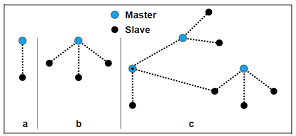
\includegraphics[scale=.7]{img/btopo.png}
\end{frame}

%%%%%%%%%%%%%%%%%%%%%%%%%%%%%%%%%%%%%%%%%%%%%%%%
\begin{frame}{Zigbee}
	\begin{itemize}\justifying{}
		\item
			IEEE 802.15 serial standards are established by IEEE 802.15 Working Group
			for Personal Area Network or short distance wireless networks.
		\item
			Zigbee is built on the IEEE 802.15.4. The two lower layers: the physical
			(PHY) layer and the medium access control (MAC) sub-layer of Zigbee stack
			architecture is pecified in IEEE 802.15.4.
	\end{itemize}
\end{frame}

%%%%%%%%%%%%%%%%%%%%%%%%%%%%%%%%%%%%%%%%%%%%%%%%
\begin{frame}{Zigbee}
	\begin{block}{IEEE 802.15.4 Features}
		\begin{itemize}\justifying{}
			\item Data rates of 250 kbps, 40 kbps, and 20 kbps. Symbol rate is 62.5 ksymbol/sspm
			\item Two addressing mode: 16-bits short and 64-bit IEEE addressing
			\item Optional use Star-topology or Peer to Peer topology, and also supposes Cluster Tree nowdays.
			\item CSMA-CA channel access
			\item Automatic network establishment by the coordinator
			\item Full handshake protocol for transfer reliability
			\item Power management to ensure low power consumption
		\end{itemize}
	\end{block}
\end{frame}

%%%%%%%%%%%%%%%%%%%%%%%%%%%%%%%%%%%%%%%%%%%%%%%%
\begin{frame}{Zigbee}
	\begin{block}{IEEE 802.15.4 Features}
		\begin{itemize}\justifying{}
			\item 16 channels in the 2.4GHz ISM band, 10 channels in the 915MHz and one channel in the 868MHz
			\item Optinal to use Acknowledgement packet
			\item Transmit Power: About 1 mW transmit power
			\item RSSI (Received signal strength indication) measurement
		\end{itemize}
	\end{block}
\end{frame}

%%%%%%%%%%%%%%%%%%%%%%%%%%%%%%%%%%%%%%%%%%%%%%%%
\begin{frame}{Zigbee}
	\begin{block}{Type of Device}
		\begin{itemize}\justifying{}
			\item RFD (Reduced Function Device)
			\begin{itemize}\justifying{}
				\item Coordinator
				\item Router
				\item End Device
			\end{itemize}
			\item FFD (Full Function Device)
			\begin{itemize}\justifying{}
				\item End Device
			\end{itemize}
		\end{itemize}
	\end{block}
	\begin{block}{IEEE 802.15.4 Topologies}
		\begin{itemize}\justifying{}
			\item Star
			\item Peer to Peer
		\end{itemize}
	\end{block}
\end{frame}

%%%%%%%%%%%%%%%%%%%%%%%%%%%%%%%%%%%%%%%%%%%%%%%%
\begin{frame}{Zigbee}
	Zigbee Topologies
	\center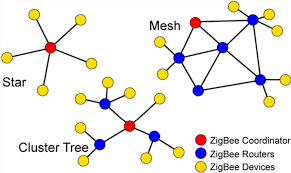
\includegraphics[scale=.7]{img/ztopo.png}
\end{frame}

%%%%%%%%%%%%%%%%%%%%%%%%%%%%%%%%%%%%%%%%%%%%%%%%
\begin{frame}{Zigbee}
	IEEE 802.15.4 MAC-PHY
	\center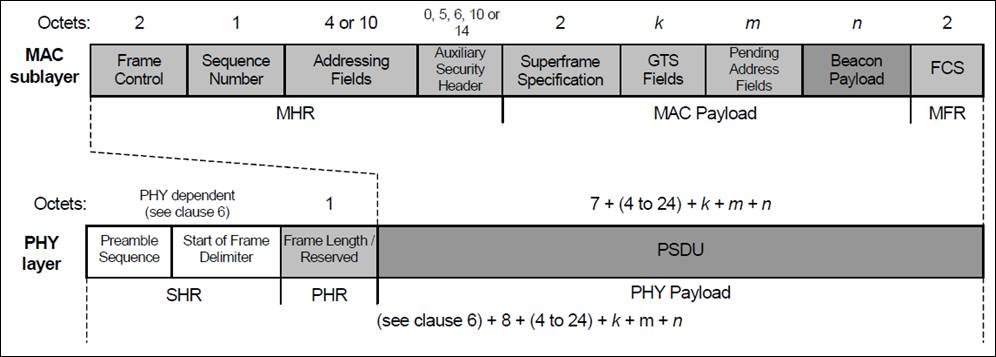
\includegraphics[scale=.4]{img/154frame.jpg}
\end{frame}

%%%%%%%%%%%%%%%%%%%%%%%%%%%%%%%%%%%%%%%%%%%%%%%%
\begin{frame}{Zigbee}
	Superframe Structure
	\begin{itemize}
		\item CAP:\@ Contention Access Period
		\item CFP:\@ Contention Free Period
		\item GTS:\@ Guaranteed Time Slots
	\end{itemize}
	\center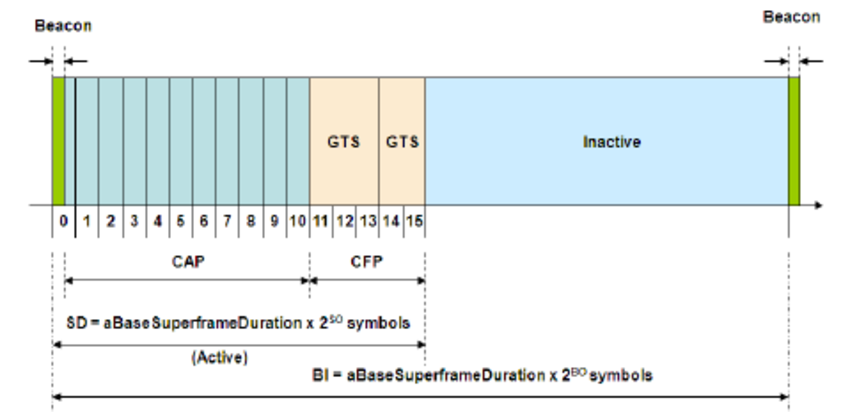
\includegraphics[scale=.3]{img/sframe.png}
\end{frame}

%%%%%%%%%%%%%%%%%%%%%%%%%%%%%%%%%%%%%%%%%%%%%%%%
\begin{frame}{Zigbee}
	Zigbee Stack
	\center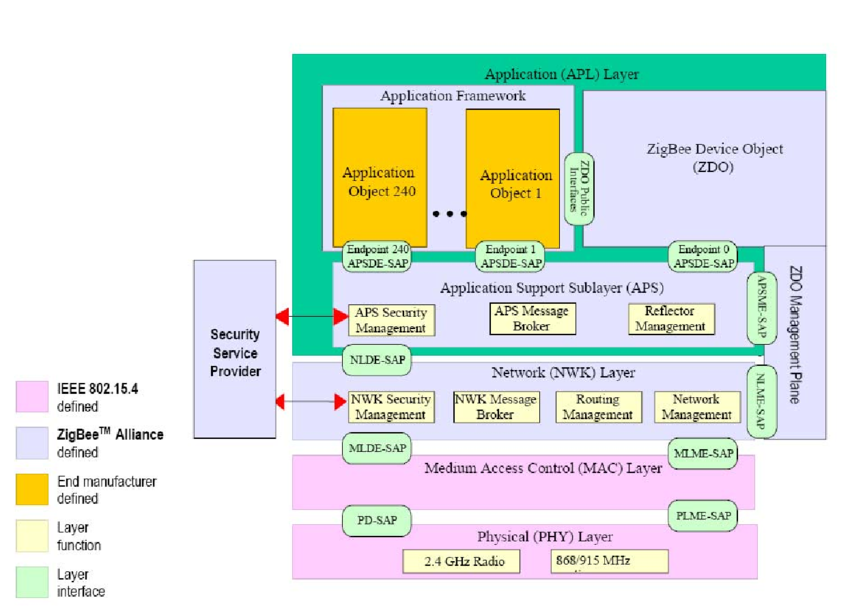
\includegraphics[scale=1]{img/zstack.png}
\end{frame}


\frame{\frametitle{Table of contents}\tableofcontents}

%%%%%%%%%%%%%%%%%%%%%%%%%%%%%%%%%%%%%%%%%%%%%%%%
\begin{frame}{A Closer look to Zigbee}
	Zigbee Problems
	\begin{itemize}\justifying{}
		\item Energy Efficiency
		\item Routing
		\item Localization
		\item Data management
		\item Reliability
		\item Security
	\end{itemize}
\end{frame}

%%%%%%%%%%%%%%%%%%%%%%%%%%%%%%%%%%%%%%%%%%%%%%%%
\begin{frame}{A Closer look to Zigbee}
	\begin{block}{An Energy Efficient Schedule for IEEE 802.15.4/Zigbee Cluster Tree WSN with Multiple Collision Domains and Period Crossing Constraint}
		\begin{itemize}\justifying{}
			\item A collision-free cluster schedule that meets all the data flows deadlines
			\item Minimization of the energy consumption of the nodes
		\end{itemize}
	\end{block}
	\footfullcite{Ahmad2018}
\end{frame}

%%%%%%%%%%%%%%%%%%%%%%%%%%%%%%%%%%%%%%%%%%%%%%%%
\begin{frame}{Zigbee}
	\center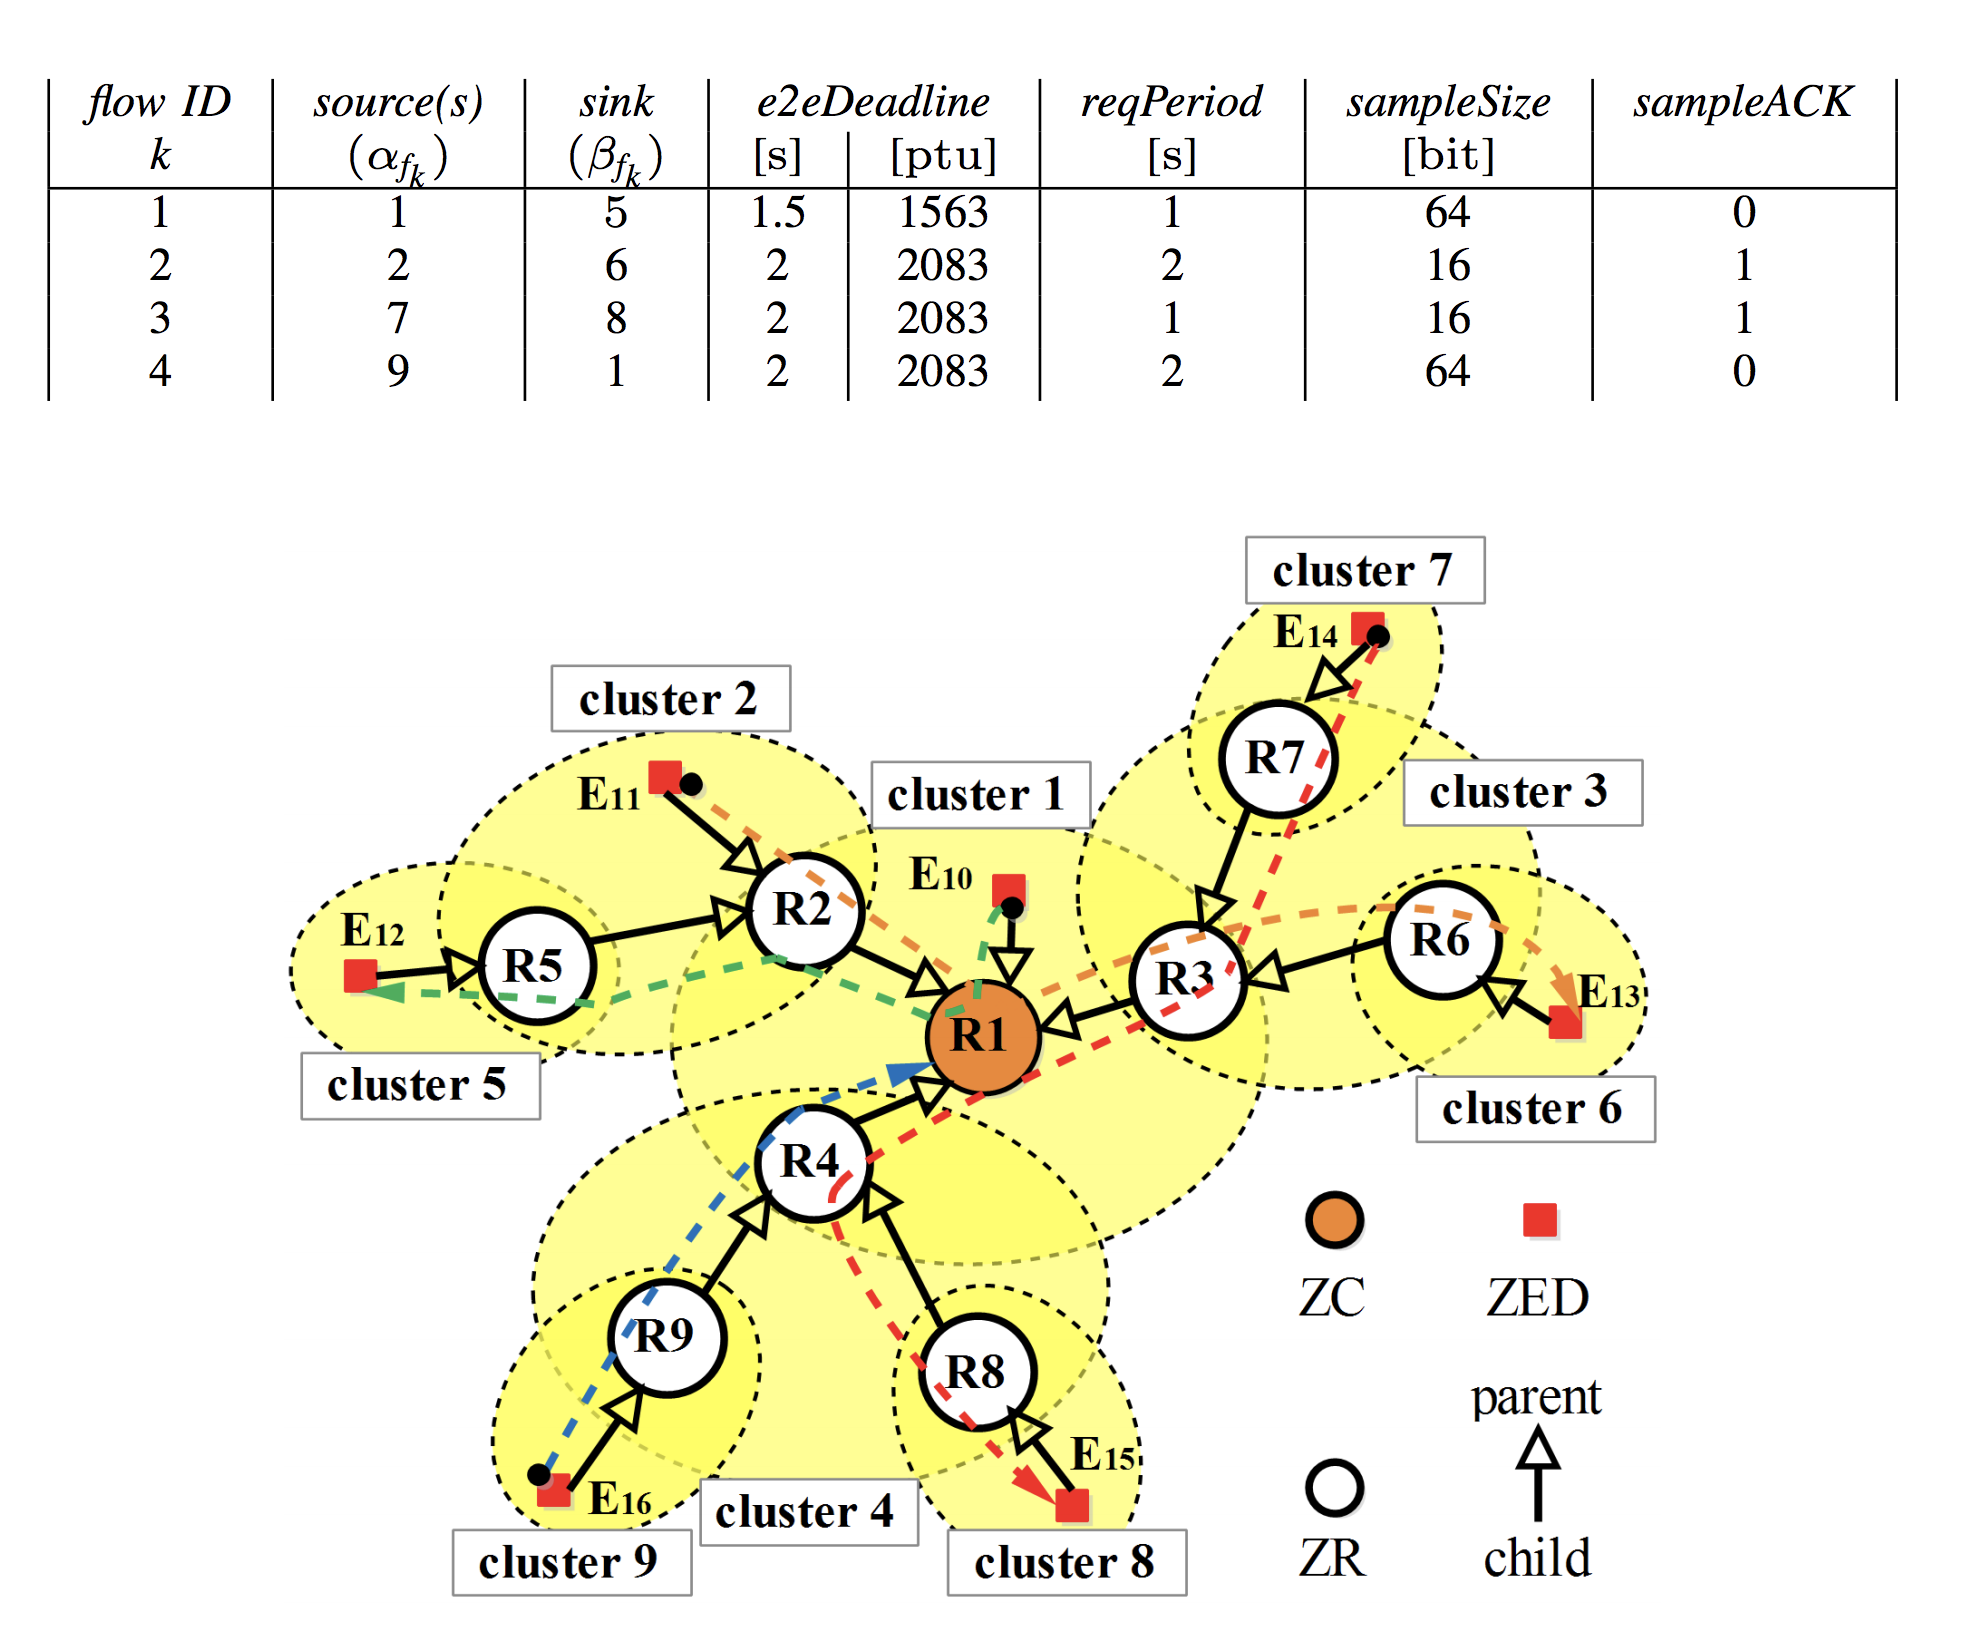
\includegraphics[scale=.2]{img/cluster-flow.png}
\end{frame}

%%%%%%%%%%%%%%%%%%%%%%%%%%%%%%%%%%%%%%%%%%%%%%%%
\begin{frame}{Zigbee}
	Average network energy consumption within 40 min
	\center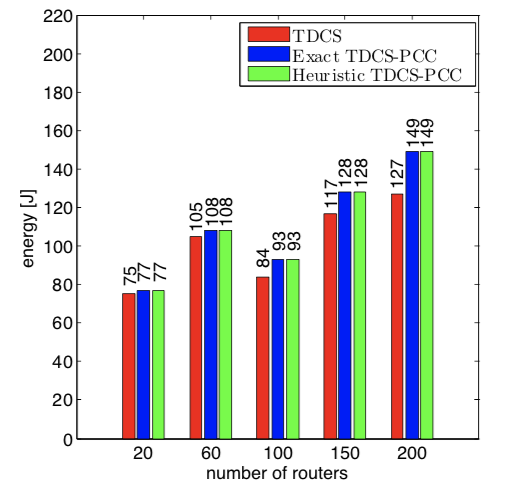
\includegraphics[scale=.5]{img/fig17.png}
\end{frame}

%%%%%%%%%%%%%%%%%%%%%%%%%%%%%%%%%%%%%%%%%%%%%%%%
\begin{frame}{Zigbee}
	Network retransmitions
	\center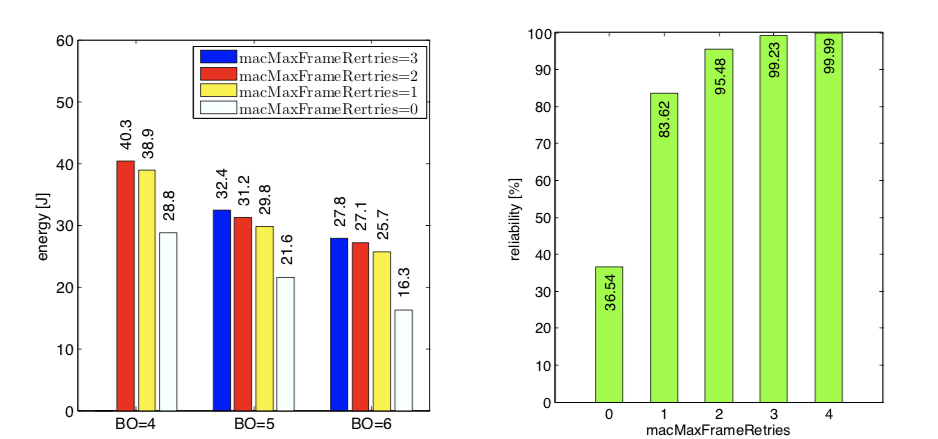
\includegraphics[scale=.5]{img/fig1819.png}
\end{frame}




\end{document}
